%%% Research Diary - Entry
%%% Template by Mikhail Klassen, April 2013
%%% 
\documentclass[11pt,letterpaper]{article}
\usepackage{float}
\newcommand{\workingDate}{\textsc{2025 $|$ April }}
\newcommand{\userName}{Charalampos Papadopoulos}
\newcommand{\institution}{National Technical University of Athens}
\usepackage{researchdiary_png}
% To add your univeristy logo to the upper right, simply
% upload a file named "logo.png" using the files menu above.

\begin{document}
\univlogo

\title{PLL Simulations Logbook}

{\Huge 8 May}\\[5mm]

\section*{Προσομοιώσεις PLL}
Στην παρούσα αναφορά θα ελέγξουμε τις δυνατότητες της υπάρχουσας υλοποίησης του PLL.
Θα το προσομοιώσουμε με την χρήση του LTSpice.

Το schematic μας είναι το εξής:
\begin{figure}[H]
  \centering
  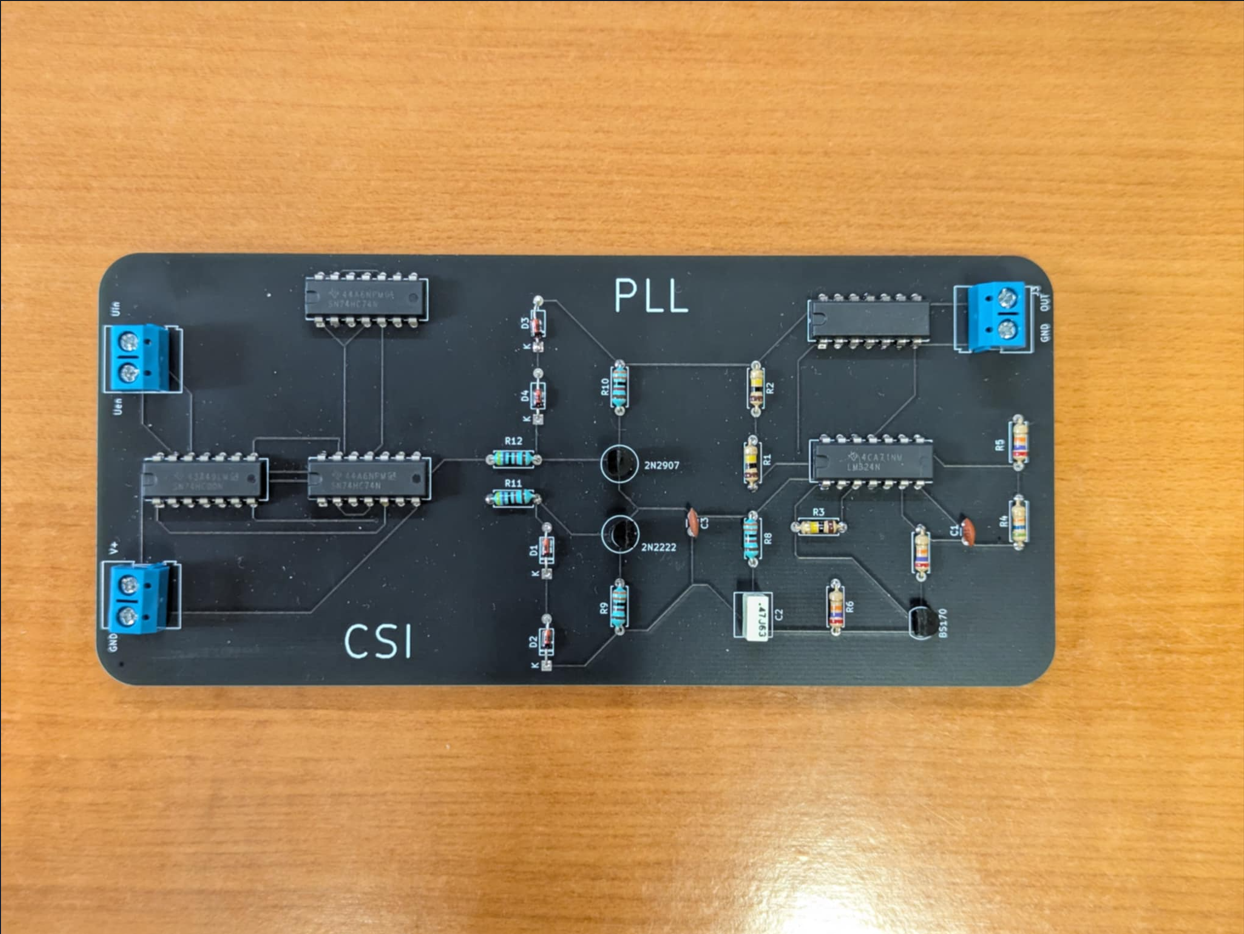
\includegraphics[width=0.8\textwidth]{PLL.png}
  \caption{PLL Schematic}
  \label{fig:pll_schematic}
\end{figure}



\end{document}